\documentclass[a4paper,11pt]{article}

\usepackage{fullpage}%
\usepackage[T1]{fontenc}%
\usepackage[utf8]{inputenc}%
\usepackage[main=francais,english]{babel}%

\usepackage{graphicx}%
\usepackage{url}%
\usepackage{abstract}%
\usepackage{amsmath}
\usepackage{mathpazo}%

\DeclareSymbolFont{Letters} {U}{zeur}{m}{n}% Euler
\DeclareMathSymbol\Gamma    {\mathalpha}{Letters}{"00}
\DeclareMathSymbol\Delta    {\mathalpha}{Letters}{"01}
\DeclareMathSymbol\Theta    {\mathalpha}{Letters}{"02}
\DeclareMathSymbol\Lambda   {\mathalpha}{Letters}{"03}
\DeclareMathSymbol\Xi       {\mathalpha}{Letters}{"04}
\DeclareMathSymbol\Pi       {\mathalpha}{Letters}{"05}
\DeclareMathSymbol\Sigma    {\mathalpha}{Letters}{"06}
\DeclareMathSymbol\Upsilon  {\mathalpha}{Letters}{"07}
\DeclareMathSymbol\Phi      {\mathalpha}{Letters}{"08}
\DeclareMathSymbol\Psi      {\mathalpha}{Letters}{"09}
\DeclareMathSymbol\Omega    {\mathalpha}{Letters}{"0A}
\DeclareMathSymbol{\alpha}  {\mathalpha}{Letters}{"0B}
\DeclareMathSymbol{\beta}   {\mathalpha}{Letters}{"0C}
\DeclareMathSymbol{\gamma}  {\mathalpha}{Letters}{"0D}
\DeclareMathSymbol{\delta}  {\mathalpha}{Letters}{"0E}
\DeclareMathSymbol{\epsilon}{\mathalpha}{Letters}{"0F}
\DeclareMathSymbol{\zeta}   {\mathalpha}{Letters}{"10}
\DeclareMathSymbol{\eta}    {\mathalpha}{Letters}{"11}
\DeclareMathSymbol{\theta}  {\mathalpha}{Letters}{"12}
\DeclareMathSymbol{\iota}   {\mathalpha}{Letters}{"13}
\DeclareMathSymbol{\kappa}  {\mathalpha}{Letters}{"14}
\DeclareMathSymbol{\lambda} {\mathalpha}{Letters}{"15}
\DeclareMathSymbol{\mu}     {\mathalpha}{Letters}{"16}
\DeclareMathSymbol{\nu}     {\mathalpha}{Letters}{"17}
\DeclareMathSymbol{\xi}     {\mathalpha}{Letters}{"18}
\DeclareMathSymbol{\pi}     {\mathalpha}{Letters}{"19}
\DeclareMathSymbol{\rho}    {\mathalpha}{Letters}{"1A}
\DeclareMathSymbol{\sigma}  {\mathalpha}{Letters}{"1B}
\DeclareMathSymbol{\tau}    {\mathalpha}{Letters}{"1C}
\DeclareMathSymbol{\upsilon}{\mathalpha}{Letters}{"1D}
\DeclareMathSymbol{\phi}    {\mathalpha}{Letters}{"1E}
\DeclareMathSymbol{\chi}    {\mathalpha}{Letters}{"1F}
\DeclareMathSymbol{\psi}    {\mathalpha}{Letters}{"20}
\DeclareMathSymbol{\omega}  {\mathalpha}{Letters}{"21}
\DeclareMathSymbol{\varepsilon}{\mathalpha}{Letters}{"22}
\DeclareMathSymbol{\vartheta}{\mathalpha}{Letters}{"23}
\DeclareMathSymbol{\varpi}  {\mathalpha}{Letters}{"24}
\DeclareMathSymbol{\varphi} {\mathalpha}{Letters}{"27}
\DeclareMathSymbol\upOmega  {\mathord}{Letters}{"0A}
\DeclareMathSymbol\upDelta  {\mathord}{Letters}{"01}


\usepackage{amssymb}



\usepackage{listings}
\usepackage{caption}

\lstset{%
	basicstyle=\sffamily,%
	columns=fullflexible,%
	frame=lb,%
	frameround=fftf,%
}%

\parskip=0.5\baselineskip

\sloppy

\author{Santiago Bautista}
\date{Juillet 2017}
\title{Sémantique et extension du langage C2QL pour la composition de techniques protégeant la confidentialité dans le nuage}

\begin{document}
\maketitle

\begin{abstract}
	Des applications de tout genre manipulent des personnelles de ses utilisateurs
	et utilisent le cloud pour s'exécuter ou s'héberger.
	Différentes techniques existent pour protéger la confidentialité de ces données.
	Pendant ce stage on a étudié la sémantique et prouvé les propriétés algébriques d'un langage permettant de décrire
	efficacement la composition de plusieurs de ces techniques, comme la fragmentation et le chiffrement.
	\begin{description}
		\item[Mots clés:]{\begin{otherlanguage}{english}
				privacy, cloud-computing, semantics, proof of correctness, algebraic laws, fragmentation, optimisation
			\end{otherlanguage}} 
	\end{description} 
	
\end{abstract}

\tableofcontents
\pagebreak

\section{Introduction}
De plus en plus de logiciels sont développés pour être exécutés dans le cloud,
et ses logiciels, de quelque sorte qu'ils soient (messagerie, gestion d'agenda personnel,
commande de pizza ou reconnaissance vocale) traitent des données personnelles, qu'ils doivent
donc protéger.

Une des propriétés qui doit être garantie dans la protection des données personnelles
est la confidentialité.
Différentes techniques existent pour protéger la confidentialité des données, 
comme par exemple le chiffrement et la fragmentation.

Dans sa thèse de 2016, Ronan Cherrueau montre que chacune de ces techniques
 a des avantages et des inconvénients,
mais qu'\emph{en composant les différentes techniques ensemble} 
on peut profiter de tous les avantages de ces
techniques en éliminant la plupart des inconvénients.
Il développe donc un langage, nommé C2QL (pour \emph{\begin{otherlanguage}{english}
		Cryptographic Compositions for Query Language
	\end{otherlanguage}}),
qui permet de décrire une telle composition de techniques de sécurisation des données
pour en vérifier la correction et raisonner plus facilement.

Le langage se présente comme un ensemble de fonctions que l'on peut
composer entre elles.
Parmi ces fonctions, il y a les fonctions classiques pour faire des requêtes
dans des bases de données, telles que la projection et la sélection, tout comme
des fonctions décrivant la protection des données, comme le chiffrement ou la fragmentation.

Un des intérêts de ce langage est que,
pour décider comment protéger les données des utilisateurs,
le développeur peut suivre un processus simple en trois étapes.
D'abord, le développeur écrit les requêtes \emph{en ne tenant compte}
ni du fait que le programme s'exécute dans le nuage, ni des mécanismes
pour le protéger.
Puis, il compose sa requête avec les fonctions de protection
nécessaires (qui dépendent du problème en particulier, des contraintes
de confidentialité spécifiques) pour avoir une requête sécurisée.
Finalement, le développeur utilise des lois de commutation entre les différentes
fonctions pour optimiser sa requête sécurisée.

Par conséquent, disposer de lois qui indiquent à quelles conditions les différentes
fonctions du langage commutent est très important.

Or, si dans sa thèse R. Cherrueau donne la plupart de ces lois,
il n'a pas eu le temps de les démontrer, ni de contempler tous les cas de figure.

C'est pourquoi, pendant ce stage, 
j'ai complété l'ensemble de lois fournies
(section \ref{compl}) dans la thèse de Ronan
et j'ai formalisé la sémantique des différentes fonctions
(section \ref{defs}) pour ensuite
démontrer la correction de ces lois (section \ref{proof}).

Une description du contexte dans lequel s'inscrit ce stage
est donnée à la section \ref{context},
et une discussion sur les aspects qui n'ont pas été traités
est donnée à la section \ref{discusion}.

\section{Contexte}
\label{context}
\subsection{De l'importance de composer les techniques de protection}

De plus en plus d'applications, en particulier
les applications web et les applications pour téléphone portable,
cherchent à utiliser le nuage, soit pour stocker du code ou des données, 
soit pour faire des calculs,
voir les deux à la fois.

En effet, le nuage peut offrir des services (que ce soit sous forme d'infrastructure,
de plateforme ou de logiciel) disposant d'une forte disponibilité et faciles à redimensionner.

Autrement dit, pouvoir utiliser le nuage est devenu un enjeu de la conception logicielle,
à cause des avantages de disponibilité et redimensionnement que cela offre.

Mais ce n'est pas le seul enjeux de la conception logicielle.

Vu que la plupart de ces applications manipulent des données personnelles, 
garantir la \emph{confidentialité} des données est également un enjeux de 
ces applications là; tout comme le sont les \emph{performances} pour garantir
une meilleure expérience à l'utilisateur de l'application.

Dans sa thèse, R. Cherrueau s'intéresse à trois techniques particulières
utilisées dans le développement logiciel et regarde comment elles interagissent
avec les trois enjeux cités plus haut.
Ces trois techniques, qu'on va décrire brièvement, sont
	le \emph{chiffrement},
	la \emph{fragmentation verticale} et
	l'\emph{exécution} de l'application \emph{chez l'utilisateur}.

\paragraph{Le chiffrement}
Lorsqu'il est bien utilisé, le chiffrement permet de garantir la confidentialité
des données de l'utilisateur.
De plus, dans certains cas, des calculs peuvent être faits sur les données chiffrées.
On appelle chiffrement homomorphe un chiffrement avec lequel on peut effectuer des calculs
avec les données chiffrées. Les chiffrement homomorphes totaux, comme celui de
Gentry (\textbf{référence à ajouter}) sont pour l'instant trop contraignants pour pouvoir être utilisés
dans la plupart des applications, mais les chiffrements homomorphes partiels,
c'est à dire les chiffrement avec lesquels on peut effectuer \emph{certaines}
opérations sur les données chiffrées, peuvent se révéler très utiles.
C'est le cas des chiffrements déterministes (dont les chiffrements symétriques)
qui sont des chiffrement homomorphes partiels, permettant le test d'égalité.

Dans tous les cas, le chiffrement implique un surcoût en terme de calculs,
donc diminue les performances. Dans certains cas, il améliore la confidentialité
et permet l'utilisation du nuage.

\paragraph{L'exécution côté client}
Si le programme était exécuté entièrement par la machine de l'utilisateur,
cela serait à la fois bon pour la confidentialité (car les données
ne seraient pas du tout exposées aux risques liés à l'utilisation du nuage
et du réseau) et pour les performances, puisque, à moins de traiter une 
trop grande quantité de données dans un calcul hautement parallélisable,
les performances du cloud sont moins bonnes que celles des machines des utilisateurs.
Par contre, l'exécution côté client ne permet pas de profiter des avantages du cloud.

\paragraph{La fragmentation verticale} consiste à séparer les différentes données
que manipule le programme entre deux clouds n'ayant aucun rapport entre eux
(à deux endroits géographiques différents, gérés par des entités différentes,
etc$\dots$).
Ceci permet de protéger celles des données personnelles qui sont constituées d'une
\emph{association} de deux données. Par exemple, dans une application stockant
un ensemble de rendez-vous, l'association $(\mathrm{date}, \mathrm{lieu})$
doit être protégée, car une personne malveillante ayant accès à ces deux
informations là à la fois pourrait suivre l'utilisateur de l'application.

La fragmentation verticale contribue à protéger la confidentialité,
mais d'une façon souvent moins forte que celles du chiffrement
ou de l'exécution côté client. Par contre, chacun des fragments
de données qu'elles génère peuvent être opérés séparément, en introduisant
ainsi, lorsque le programme le permet, une dose de parallélisation
supplémentaire qui peut améliorer les performances et permettre de tirer
encore plus d'avantages du nuage.

\begin{figure}
	\begin{center}
		
\includegraphics[width=0.7\textwidth]{snps.png}
		\caption{Enjeux et techniques dans le cloud-computing}
		\caption*{(image provenant de la thèse de Ronan Cherrueau)}
		\label{enjeux}
	\end{center}
\end{figure}

La figure \ref{enjeux} résume comment ces trois techniques
là interagissent avec les trois enjeux cités plus haut.

Dans sa thèse, Ronan Cherrueau montre qu'en composant ces différentes techniques
on peut à la fois profiter des avantages du nuage, protéger la confidentialité
et améliorer les performances d'un programme.

Pour pouvoir décrire comment s'effectue une telle composition,
pour pouvoir vérifier la correction d'une telle composition et
pour pouvoir raisonner dessus, Cherrueau a introduit un langage: C2QL.

\subsection{Un langage pour décrire la composition: C2QL}
Le langage C2QL donne une façon d'exprimer comment les techniques
mentionnées ci-dessus se composent avec les fonctions classiques de l'algèbre relationnelle.

Les données manipulées sont donc représentées sous forme de tables, ou relations,
c'est à dire un ensemble de lignes contenant des valeurs pour chacun(e) des 
différent(e)s attributs ou colonnes considéré(e)s.

Dans l'exemple de l'application stockant des rendez-vous, cette
table contiendrait autant de lignes que de rendez-vous stockés 
dans l'application et (par exemple) trois colonnes ou attributs: 
nom de l'utilisateur
ayant stocké le rendez-vous, date du rendez-vous et lieu du rendez-vous.

\paragraph{Les opérateurs empruntés à l'algèbre relationnelle}
présents dans ce langage sont
\begin{itemize}
	\item La projection, notée $\proj$ 
	qui consiste à ne considérer que certains des attributs de la table.
	\item La sélection, notée $\sel$
	qui consiste, pour une table donnée, à ne considérer que
	les lignes satisfiant un certain prédicat.
	\item La jonction naturelle, notée $\Join$, qui combine
	les informations de deux tables en fonction des attributs qu'elles ont
	en commun.
	\item L'aggrégation et la réduction
	(notées respectivement $\group$ et $\operatorname{fold}$)
	permettant, respectivement, 
	de regrouper les lignes qui partagent les mêmes valeurs
	pour un certain ensemble d'attributs
	et d'effectuer des opérations sur les groupes de lignes ainsi obtenus.
\end{itemize}

\paragraph{Les opérateurs relatifs à la protection des données}
présents dans le langage sont
\begin{itemize}
	\item La fragmentation verticale, notée $\frag$,
	qui sépare une table en deux tables: la première contenant certains
	des attributs (colonnes) de la table d'origine, et la deuxième contenant
	le reste des attributs de la table d'origine.
	
	\item La défragmentation verticale, notée $\defrag$,
	qui effectue l'opération inverse: à partir de deux
	tables n'ayant pas d'attributs en commun, reconstruit une seule table.
	Un attribut spécial, $id$, servant à identifier chaque ligne et créer lors de 
	la fragmentation d'une table, rend la défragmentation possible.
	
	\item Le chiffrement, noté $\operatorname{crypt}$
	qui chiffre un attribut dans une table.
	
	\item Le déchiffrement, noté $\operatorname{decrypt}$
	qui déchiffre un attribut dans une table.
\end{itemize}

\paragraph{\og Où est passée le calcul côté client?\fg{}}
est peut-être une question que vous vous posez peut-être en ce moment.
La raison pour laquelle il n'y a aucun opérateur dans C2QL 
qui permette d'exprimer le rapatriement des données sur la machine de l'utilisateur
est que cette gestion est faite implicitement, pour garantir
que les requêtes C2QL protègent toujours la confidentialité, par conception.
En effet, dans le langage C2QL on suppose que les données à protéger sont toujours
soit un attribut, dans lequel cas il peut être protégé par chiffrement,
soit une association de deux attributs, dans lequel cas elle peut être protégée
par fragmentation. Par conséquent, dans une requête, le premier déchiffrement 
ou la première défragmentation (ou l'absence de chiffrement ou de
fragmentation dans des cas où ils auraient été nécessaires)
brisent la protection des données et requièrent que
les données soient rapatriées chez l'utilisateur pour cette opération et toutes
les opérations postérieures.

Ainsi, on peut, en regardant une expression C2QL et en connaissant les
contraintes de confidentialité à respecter,
déduire à quel moment les données doivent être rapatriées chez l'utilisateur;
sans que cette opération aie besoin d'apparaître explicitement dans l'expression.

\textbf{Rajouter un exemple serait probablement utile}

\textbf{TODO Expliquer les contraintes de sécurité avant l'aspect implicite
	du c.c.}

Ce langage a été défini comme un Langage de Domaine Spécifique Embarqué dans
Idris, qui est un langage à types dépendants.
Le système de typage d'Idris et les types donnés aux opérateurs permettent
de vérifier, lorsqu'on écrit une requête en C2QL que celle-ci aura un sens
au moment de l'exécution.

\subsection{Utiliser C2QL: commuter les opérateurs}
Dans sa thèse, Cherrueau expose un méthode pour se servir facilement
et efficacement de C2QL, en trois étapes.

\paragraph{Première étape: écrire la version locale de l'application.}
Le développeur peut commencer par écrire les requêtes de son application
sans tenir compte de l'utilisation du cloud ni de la protection
des données. C'est ce qu'on appelle ici une version \og locale \fg{}
du programme; c'est le programme tel qu'il pourrait s'exécuter dans la machine de l'utilisateur, localement.
Cette version de l'application est beaucoup plus facile à écrire 
qu'une version utilisant efficacement les techniques de protection.

\paragraph{Deuxième étape: ajouter les techniques de protection nécessaires.}
Le langage C2QL suppose que les contraintes de confidentialité sont de deux types:
soit il s'agit d'une association entre deux attributs que l'on veut 
protéger, dans lequel cas on choisit de mettre les deux attributs de l'association
dans des fragments distincts grâce à la fragmentation verticale, soit il s'agit de la
valeur d'un attribut que l'on veut protéger, dans lequel cas soit on chiffre cette valeur,
soit on la décompose sur plusieurs fragments avec la technique exposée par Aggarwal 
(\textbf{TODO rajouter la référence}). Dans les deux cas on peut passer des 
versions locales des requêtes à des versions protégées en faisant apparaître 
à droite de la requête les fonctions de protections composées avec leurs fonctions réciproques.

\paragraph{Troisième étape: faire commuter les différentes fonctions.}
En faisant commuter les différents opérateurs qui apparaissent dans les requêtes,
on peut aboutir à une requête optimisée, profitant des avantages du cloud et de bonnes performances.
Pour cela, on a besoin de savoir à quelles conditions les différents opérateurs de C2QL peuvent
commuter.

C'est sur cet ensemble de lois qui indiquent à quelle condition deux fonctions de C2QL peuvent
commuter que je me suis intéressé pendant mon stage.

\section{Contribution}
Dans mon travail avec l'ensemble de lois de C2QL,
j'ai commencé par poser une sémantique formelle pour les différentes fonctions
du langage C2QL (section \ref{defs}),puis j'ai complété cet ensemble de lois,
en m'intéressant à toutes les combinaisons possibles de lois que l'on pouvait
vouloir commuter dans le langage (section \ref{compl}), ensuite 
j'ai démontré la correction sémantique de ces lois-là (section \ref{proof})
et en ce moment je travaille sur l'automatisation de l'optimisation 
des requêtes, en réfléchissant à comment déterminer, parmi les commutations possibles,
lesquelles il faut choisir pour optimiser une requête (section \ref{opti}).

\subsection{Établir des définitions}
\label{defs}
Les définitions des différents opérateurs présentes dans la thèse de 2016
sont données en français, ce qui facilite leur compréhension, mais rend
impossible une preuve mathématique de la correction des lois les concernant.

J'ai donc commencé par poser des définitions formelles des fonctions du langage
C2QL.

Pour former ces définitions, j'ai du faire des choix à plusieurs reprises.
À chaque fois, j'ai utilisé les deux mêmes critères pour guider mes choix:
d'une part il faut que les définitions que je choisi permettent au langage
d'être le plus expressif possible, d'autre part il faut que les définitions
choisies facilitent une démonstration rigoureuse de la correction
des lois de commutation.

Pour un document contenant l'ensemble des définition,
se référer à l'annexe A.

Dans ce rapport je vais me centrer principalement
sur celles des définitions où il y a eu des choix à faire
(en exposant les motivations qui ont permit d'effectuer un choix
plutôt qu'un autre) et celles des définitions où il y a des différences par rapport
aux définitions qui étaient suggérées par les notations de la thèse,
en expliquant les motivations de ces différences.

\subsubsection*{Des tuples ou des fonctions?}
Dans son livre de 1982, Ullman parle de deux
façons de définir les relations (tables) de l'algèbre relationnelle:
soit comme un sous-ensemble d'un produit de domaines
(donc comme un ensemble de tuples, où chaque
tuple représente une ligne
de la table et chaque coordonnée de chaque tuple correspond
à la valeur pour un attribut donné), soit comme un ensemble de fonctions
définies sur l'ensemble des attributs (chaque fonction correspond donc
à une ligne de la table, et la valeur d'un attribut pour une ligne donnée
est son image par cette fonction).

Ullman décide d'utiliser la première définition pour le reste de son livre,
et ne détaille pas plus la deuxième définition. C'est pourtant cette deuxième
définition que j'ai décidé de prendre dans ce cas ci, puisque que ce soit
pour le chiffrement comme pour la fragmentation, on fait ici référence aux différentes
colonnes d'une table par leur nom (toutes les colonnes ont un nom, et tous les
noms des colonnes sont différents) et il est donc plus facile de raisonner,
par exemple, sur la fragmentation, avec cette définition-là:
en effet, la fragmentation se définit alors en thermes de simples restrictions
sur certains ensembles.

Ainsi, la définition d'une relation que j'ai retenue a été la suivante
(où $\val$ est un ensemble appelé ensemble des valeurs):

\begin{defi*}
	On appelle \emph{relation} de schéma relationnel $\Delta$
	tout ensemble de fonctions de $\Delta \cup \{ id \}$ dans $\val$.
\end{defi*}

\subsubsection*{Expressivité ou prudence?}
Lorsqu'on définit un langage et sa sémantique, il faut entre autres
décider quelles expressions appartiennent au langage
(ou \og ont du sens\fg{}) et lesquelles n'y appartiennent pas.

Face à ce choix, deux attitudes sont possibles.
Soit on favorise l'expressivité du langage en donnant du sens
au plus d'expressions possibles, soit on est \guillemets{prudent}, restrictif,
en ne donnant du sens qu'à un ensemble restreint d'expressions.

L'avantage de l'approche restrictive est qu'elle évite des erreurs de programmation
où le développeur se retrouve à écrire quelque chose dont le sens
ne correspond pas à celui qu'il désirait.

Dans l'implémentation de C2QL en tant que langage embarqué dans Idris
que R. Cherrueau a développé en 2016, c'est l'approche
\og prudente \fg{} qui est privilégiée.

Cependant, je me suis aperçu que, du fait que l'implémentation
déjà existante privilégie un langage restrictif,
les définitions que je pose peuvent définir un langage plus
expressif sans que cela enlève
les avantages du langage restrictif.

En effet, si jamais une loi de commutation est correcte avec des définitions
moins restrictives, le sens de la requête reste le même avant et après
commutation et donc la loi de commutation est également sémantiquement correcte pour
les définitions plus restrictives.

\subsubsection*{Des sélections portant sur plus d'un attribut à la fois.}
Dans certaines des lois présentes dans la thèse, la notation
suggère que les prédicats utilisés lors des filtrages ne portent que sur
un seul attribut à la fois.

Ainsi, par exemple, dans la loi (7) à la page 30 de la thèse
concernant la commutation entre la jointure naturelle et la
sélection,
on lit
\begin{align*}
\sel_{p\alpha \wedge q\beta} \circ \Join 
& \equiv \Join \circ (\sel_{p\alpha}, \sel_{q\beta})
& \text{si $\alpha \in \Delta$ et $\beta \in \Delta'$}
\end{align*}
où $\Delta$ et $\Delta'$ représentent respectivement le schéma relationnel
du premier argument et le schéma relationnel du deuxième argument.

Cette notation suggère que les prédicats $p$ et $q$ portent
chacun sur un seul attribut (respectivement $\alpha$ et $\beta$).

Le problème est qu'il y a certains prédicats qui ne peuvent
pas ce décomposer en des prédicats portant chacun sur un seul attribut.

Par exemple, si on dispose d'une base données concernant
des ornithorynques, qu'un des attributs de la base de données indique
la date où l'ornithorynque a vu un kangourou pour la première fois,
et qu'un autre des attributs indique la date où l'ornithorynque a pondu des oeufs
pour la première fois,
et que l'on ne veut s'intéresser qu'aux ornithorynques ayant vu des kangourous avant
de pondre des œufs pour la première fois, alors le prédicat
("date de première vision d'un kangourou" < "date de première ponte des oeufs")
ne peux pas être décomposé en deux prédicats qui porteraient l'un sur 
la date de la première vision d'un kangourou et l'autre sur la date de la 
première ponte d'œufs.

Ainsi, dans ma définition de ce qu'est une sélection et ce qu'est un prédicat,
j'ai supposé que la valeur de vérité d'un prédicat dépendait de plusieurs
attributs à la fois, et pour refléter cela j'utilise la notion de
\emph{domaine d'un prédicat}.

\begin{defi*}
On appelle \emph{domaine} d'un prédicat $p$ le plus petit
	ensemble $D$ tel que:
	$$
	\forall (l, l') \in \ls^2, (l|_D = l'|_D \Rightarrow  p(l) = p(l')) 
	$$
	et on le note $\dom(p)$.
	
	(Où $\ls$ est l'ensemble de toutes les lignes possibles.)
\end{defi*}

Avec cette définition là, la loi de commutation entre la jonction
et la sélection devient
\begin{align*}
\selP \circ \Join
& = \Join \circ (\selP, \id)
& \text{si $\dom(p) \subset \delta_1$}
\label{seljoin1}\\ 
\selP \circ \Join
& = \Join \circ (\id, \selP)
& \text{si $\dom(p) \subset \delta_2$}
\end{align*}
(où $\delta_1$ et $\delta_2$ sont les schémas relationnels de, respectivement,
le premier et le deuxième argument).

\subsubsection*{Compter, ou agréger et réduire?}
Le développeur peut vouloir agir sur plusieurs lignes à la fois.

Le choix qui a été fait dans la thèse, c'est de traiter l'exemple
de la fonction \lstinline|count|, qui permet de regrouper, \emph{en les comptant},
les lignes ayant les mêmes valeurs pour un certain ensemble d'attributs.

Je me suis posé la questions de savoir si les opportunités d'optimisation
exposées dans la thèse par rapport à la fonction \lstinline|count| et à sa façon de commuter
avec les autres fonctions lui étaient propres, ou si elles étaient généralisables
à toutes les fonctions d'agrégation. Plutôt que de m'intéresser à la fonction
\lstinline|count|, je me suis donc intéressé 
aux fonctions \lstinline|group| et \lstinline|fold|, qui permettent
de regrouper, \emph{en appliquant une fonction quelconque aux autres attributs},
les lignes ayant les mêmes valeurs pour un certain ensemble d'attributs.

En faisant cela, j'ai remarqué que les optimisations proposées pour la fonction
\lstinline|count| ne lui sont pas propres et se généralisent bien aux
fonctions \lstinline|group| et \lstinline|fold|.

\paragraph*{Remarque}
Pour pouvoir vraiment exprimer la fonction \lstinline|count|
à l'aide des fonctions \lstinline|group| et \lstinline|fold|
il faudrait également introduire des fonctions permettant d'ajouter ou de 
renommer des colonnes aux/des relations manipulées.
Or, comme le fait remarquer Cherrueau dans sa thèse en citant Ullman,
\og The nonquery aspects of a query langage are often straighforward\fg{}.
L'ajout et le renommage d'attributs n'en sont pas l'exception:
leur intéraction avec les autres fonctions du langage ne présente 
\emph{a priori} aucune difficulté particulière, et donc ces deux opérations-là
n'ont pas été traitées.

\subsubsection*{Défragmentation et jointure, un air de famille trompeur}
Dans un premier temps, nous avons voulu voir la défragmentation comme un cas
particulier de jointure naturelle, où l'attribut en commun entre
les deux relations serait l'identifiant
des lignes.

Cependant, il s'est avéré que ce n'était pas possible de traiter la défragmentation
comme un cas particulier de jointure, car, du fait que la jointure
peut produire plusieurs lignes là où avant il n'y en avait qu'une seule,
la jointure ce doit de changer les identifiants des lignes pour des identifiants frais,
ce qui est incompatible avec le comportement qu'a la défragmentation
vis-à-vis des identifiants des lignes.

Ainsi, il a été nécessaire de créer des définitions séparées pour ces deux notions.

\subsection{Compléter les propriétés}
\label{compl}
Pendant ce stage, j'ai également cherché à compléter l'ensemble des lois de commutation.

J'ai choisi comme critère de complétude le fait que tous les couples de fonctions
du langage (tous les cas de figure possibles où l'on pourrait vouloir commuter
deux fonctions) soient envisagés.

\begin{figure}
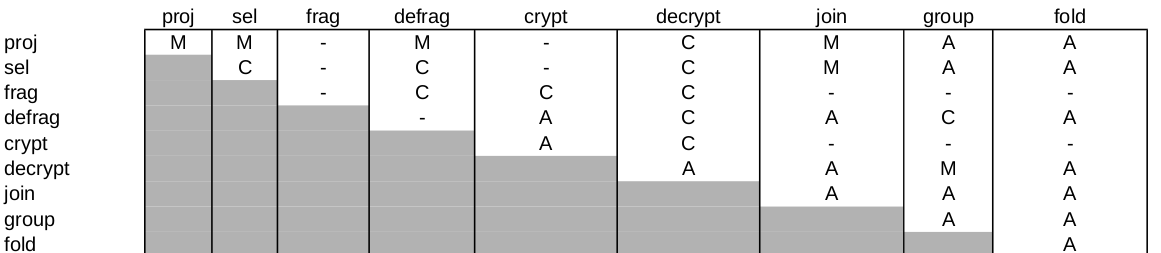
\includegraphics[width=\textwidth]{complLoisBilan.png}
\caption{Bilan des lois conservées (C), modifiées (M) et ajoutées (A)}
\label{complLois}
\end{figure}

Le tableau de la figure \ref{complLois}  montre quelles lois étaient déjà
présentes dans la thèse de 2016 ou dans l'article de 2015 de R. Cherrueau
et ont été conservées (marquées avec un \emph{C}),
quelles lois nous avons modifiées (marquées avec un \emph{M}),
quelles lois nous avons rajoutées (marquées avec un \emph{A})
et quelles lois n'ont pas à être considérées dans l'approche qui est celle
de C2QL (marquées d'un tiret \og - \fg{}).

Pour un document contenant l'ensemble des lois après ce stage,
se référer à l'annexe B.


\subsection{Prouver les propriétés}
\label{proof}
Pour pouvoir utiliser les lois de commutation
pour créer des programmes C2QL optimaux,
il est nécessaire de s'assurer que ces lois sont correctes,
c'est à dire que le résultat obtenu avant et après la
commutation des opérateurs est bien le même.

Pour démontrer la correction des lois de commutation,
deux approches sont possibles:
soit nous essayons de les démontrer à la main,
soit nous essayons de les démontrer de façon automatique
avec un \emph{prouveur} ou un \emph{assistant de preuve}
tel que \typeT{Coq}.

Nous avons opté pour la première approche,
principalement pour des raisons de temps.
En effet, vu qu'il s'agit d'un stage de L3
nous n'avons aucune expérience dans l'utilisation
des prouveurs ou des assistants de preuve,
et donc un temps non négligeable aurait été nécessaire
à la prise en main de tels outils.
Or, l'appropriation du sujet et du langage C2QL
avaient déjà pris un temps certain, donc
nous n'étions pas sûrs d'avoir le temps nécessaire.
Ceci est d'autant plus vrai que nous n'avions
aucun moyen de nous assurer que les méthodes 
de preuves automatiques (ou semi-automatiques) seraient
adaptés au problème en question.

\textbf{La structure des preuves} est,
à quelques exceptions près, toujours la même.
En effet, il s'agit, de montrer que pour deux fonctions
$f$ et $g$ du langage C2QL, les fonctions
$f \circ g$ et $g \circ f$ sont, selon le cas,
égales ou équivalentes.

Pour cela la méthode suivie est de considérer une relation
(ou un tuple de relations) $r$ quelconque et de montrer
que $(f \circ g) (r)$ est égal (ou équivalent)
à $(g \circ f) (r)$.

Mis à part certains cas où la fonction
$\frag$ intervient,
$(f \circ g) (r)$ et $(g \circ f) (r)$ sont tous les deux
des ensembles (finis), et donc pour prouver leur égalité
(ou leur équivalence) soit on prouve qu'ils sont
l'un inclus dans l'autre et l'autre inclus dans l'un,
soit on prouve que l'un est inclus dans l'autre et qu'ils
ont tous deux même cardinal.

\paragraph{Égalité ou équivalence}
La plupart du temps, c'est bien d'une égalité qu'il s'agit
entre les deux résultats en question.
Cependant, on va ci-dessous expliquer pourquoi
lorsque l'une des fonctions qu'on cherche à faire commuter
est la fonction de jonction, on ne peux pas parler
d'égalité proprement dite et il faut parler d'équivalence.

Cela vient de la gestion des identifiants des lignes.
Pour pouvoir défragmenter des relations issues d'une
fragmentation, on utilise des identifiants pour les lignes:
au sein de chacune des relations manipulées, chaque ligne
possède un identifiant qui (dans la relation) 
lui est unique.
Ainsi, lors de la fragmentation, les deux morceaux
d'une ligne gardent le même identifiant,
ce qui permet de les faire correspondre lors de la 
défragmentation.
Comme au sein de chaque relation chaque identifiant
est unique, cette correspondance se fait sans ambiguïté;
c'est bien le comportement désiré.

Cependant, lors d'une jointure, une ligne d'une des tables
jointes peut donner lieu à plusieurs lignes dans
le résultat, et il faut bien que ces lignes-là aient
un identifiant
(dans le cas où l'on voudrait les fragmenter par
la suite). Or cet identifiant ne peut pas correspondre
à celui de l'une des lignes qui lui a donné naissance,
parce qu'il ne serait alors pas unique.
Il ne peut pas non plus correspondre à un couple
avec les deux identifiants des deux lignes lui ayant
donné naissance, car une autre jonction
(avec un ensemble différent d'attributs en communs,
par exemple après une projection) pourrait donner
lieu, ailleurs dans le système,
à des lignes ayant le même identifiant que la ligne
crée par la jonction, sans que ces deux lignes aient
un rapport entre elles.

Ainsi, les effets propres à la jonctions nécessitent
que lors d'une jonction, les lignes du résultat 
aient des identifiants frais, qui ne soient
présents nulle part ailleurs dans le système.

Une conséquence directe de cela, est que
les lois de commutation ne peuvent pas assurer l'égalité
stricte des résultats lorsqu'une jonction intervient,
car la jonction crée un identifiant frais pour chaque
ligne résultat, et que deux identifiants frais
(ceux de chaque résultat) n'ont aucune raison d'être
égaux entre eux.

Dans ces cas-là il s'agit donc de prouver une 
égalité \emph{aux identifiants des lignes près}.
C'est ça qu'on appelle \emph{équivalence}.

\subsection{Optimiser les requêtes}
\label{opti}
Une partie importante dans le développement des
applications C2QL est le passage d'une requête
sous sa forme locale (sans tenir compte
du fait qu'elle s'exécute dans le cloud,
ni tenir compte des mécanismes de protection utilisés)
à une version optimisée.

En effet, tout l'intérêt du langage C2QL est d'obtenir
un programme tirant avantage de la composition
pour être particulièrement performant
(au sens des trois critères définis dans la section
\ref{context}) tout en facilitant au maximum
le développement pour le développeur
(en lui permettant de n'écrire que la version locale
des requêtes).

C'est l'utilisation des lois de commutation qui permet
de passer de la version locale à la version
optimisée, mais cette utilisation se fait pour le moment à
la main: à chaque étape, le développeur doit regarder, 
dans les lois applicables, laquelle il veut appliquer.

Pour faciliter la tache au programmeur, on peut
vouloir automatiser ce processus d'optimisation,
ce qui pose plusieurs questions.

\paragraph{Choix des métriques}
Les lois, peuvent avoir des effets sur les trois
objectifs/critères suivants:
\begin{itemize}
	\item Utiliser le cloud le plus possible
	\item Utiliser le moins de temps possible
	\item Faire transiter le moins de données
	possibles à travers le réseau
\end{itemize}
Ainsi donc, si jamais on doit choisir entre deux lois de commutation différentes applicables à une requête donnée
et mutuellement exclusives; pour faire un choix objectif
il faut disposer d'une manière de mesurer l'effet produit
par chacune de ces lois par rapport à ces critères-ci.

Qui plus est, si les lois parmi lesquelles il faut choisir
agissent sur des critères différents, il
peut être nécessaire de pouvoir comparer l'importance des
différents critères entre eux. Autrement dit,
si l'on dispose d'une métrique pour chaque critère,
il faut avoir une façon d'en déduire une métrique
globale. Ceci peut nécessiter de s'intéresser aux
nécessités et visées spécifiques de l'application en question.

\paragraph{Choix de la méthode d'exploration}
Les différentes suites de lois appliquées
pour optimiser une requête se présentent comme
un arbre de transformations possibles, qu'il faut donc
explorer pour trouver la forme la plus optimale
pour la requête.

Il faut donc choisir une méthode d'exploration
pour explorer l'arbre en question.

\paragraph{Une première approche, naïve}
En ce moment, nous sommes en train de développer
une toute première approche, complètement naïve
d'un optimiseur automatique de requêtes C2QL.
La méthode d'exploration choisie est l'exploration
exhaustive. La métrique choisie consiste en,
pour chaque lois et chaque critère, affecter un score
de 1, 0 ou -1 selon le fait que la loi favorise,
soit neutre, ou défavorise le critère en question;
et on affecte la même importance, le même poids,
aux métriques des trois critères, par une simple somme,
pour obtenir la métrique globale.

%%
\section{Travail futur}
\label{discusion}
Comme nous l'avons vu dans la section
\ref{contrib}, le but de ce stage 
était surtout de gagner en assurance et en
\og complétude \fg{} sur un aspect précis
du langage C2QL: l'ensemble de lois
de commutation qui permettent de passer d'optimiser une
requête C2QL.

Ce but-là a été réussi, mais il reste, en ce qui
concerne le langage C2QL, des ajouts et
approfondissements intéressants qui peuvent être faits
(tels que l'ajout d'un compilateur vers une application
concrète ou la prise en compte d'autres critères de
sécurité et d'autres mécanismes de sécurité), et,
en ce qui concerne le travail de ce stage, 
l'automatisation de l'optimisation de requêtes,
qui n'a été que effleurée, pourrait être traitée
de façon plus approfondie.

\subsection*{Un compilateur concret de C2QL}
Pour l'instant, C2QL dispose d'une implémentation
en tant que langage embarqué dans Idris; qui permet
de vérifier certaines propriétés de \og bonne formulation
\fg{} des requêtes qu'on écrit en C2QL. Par exemple,
lorsque, dans une requête, on déchiffre
un attribut, l'implémentation actuelle
vérifie que l'attribut en question était bien chiffré.
Ce genre de vérifications permet d'éviter un certain
nombre d'erreurs de programmation.

Pour information, Idris est un langage avec des types
dépendants, ce qui veut dire qu'en Idris, le type
des variables peut dépendre d'une ou plusieurs valeurs.
Ainsi, on peut préciser comme type 
\og Liste avec 3 éléments \fg{} et ce type là
\emph{dépend} de la valeur 3.
Mais les valeurs dont dépend un type ne doivent pas
forcément être constantes. Le type d'une variable peut
en effet dépendre de la valeur d'une autre variable,
ou même du résultat de l'application d'un certain type
de fonction, les fonctions \emph{totales}, à une variable.
Pour faire simple, une fonction est dite \emph{totale}
en Idris, si Idris est capable de vérifier statiquement
que cette fonction termine.
Par exemple, le calcul de la longueur d'une liste peut
être implémenté de façon totale, et donc
\og un couple de listes de même longueur \fg{}
peut très bien être un type en Idris.

Grâce à l'utilisation de types dépendants en Idris,
en typant les requêtes avec les schémas relationnels
des relations utilisées,
l'implémentation actuelle de C2QL peut vérifier
de façon fiable des propriétés qui seraient autrement
plus difficiles à obtenir.

\textbf{Cependant}, même si l'implémentation
actuelle permet d'exprimer les requêtes à effectuer
et d'en vérifier des propriétés; elle n'offre aucun moyen
d'exécuter concrètement ces requêtes sur des
vraies données.
Il a été envisagé par l'auteur de la thèse
de réaliser un compilateur qui transforme un programme
C2QL (i.e. un ensemble de requêtes C2QL) en
des programmes écrits par exemple en JavaScript
pour être exécutés l'un par la machine du client,
les autres par les différents clouds concernés.
Un travail futur pourrait consister en l'élaboration
d'un tel compilateur de C2QL vers une application
\og concrète \fg{}, exécutable sur le cloud.

De la même façon,
l'auteur de la thèse avait envisagé de
créer un \og compilateur \fg{} de C2QL vers
ProVérif pour pouvoir, avec ProVérif,
vérifier que le programme C2QL écrit respecte bien
les contraintes de confidentialité qui avaient été fixées.

Il existe actuellement une transformation de
C2QL vers le pi-calcul; il resterait donc
à créer une transformation du pi-calcul vers ProVérif.

\subsection*{Un optimiseur réaliste des requêtes}
Comme mentionné dans la section \ref{opti},
l'optimiseur automatique de requêtes
que nous sommes en train de développer 
suit une approche naïve (tantôt dans sa façon de
mesurer l'effet de l'application d'une commutation, 
comme dans l'exploration des suites de commutations
possibles) et a pour seule ambition d'être une
première approche.

Un travail futur pourrait être de créer un optimiseur
de requêtes plus réaliste; ce qui nécessiterait
une réflexion plus approfondie, en particulier
en ce qui concerne les métriques permettant d'estimer
l'effet d'une commutation donnée.

\subsection*{D'autres critères et mécanismes de sécurité}
C2QL est un langage qui permet d'exprimer la composition 
de différents mécanismes de sécurité, comme on l'a vu dans
la section \ref{descrC2QL}.

Les trois mécanismes de sécurité actuellement
pris en compte dans C2QL
(le chiffrement, la fragmentation verticale
et le fait de réaliser les calcul sur
la machine du client)
sont tous les trois des mécanismes permettant
de protéger la \emph{confidentialité} des données.

Or, la confidentialité n'est pas le seul critère
de sécurité que l'on peut vouloir garantir.
L'intégrité des données ou la disponibilité des données,
par exemple, peuvent également être des critères 
de sécurité importants; et pour les satisfaire,
il est nécessaire de prendre en compte d'autres
mécanismes de protection.

Par exemple, le tatouage des données 
(qui consiste à altérer légèrement les données,
à en ajouter une \og marque \fg{}) peut être utilisé
pour protéger l'intégrité des données.
En effet, si la marque en question constitue une
signature électronique, alors toute attaque voulant porter
atteinte à l'intégrité des données (en remplaçant les 
vraies données par des fausses données) serait
repérable par une vérification de la marque
associée à ces données là.

Ajouter d'autres mécanismes de sécurité
(tels que le tatouage) pour prendre en compte
d'autres critères de sécurité (tels que l'intégrité)
serait une extension possible du langage C2QL.

\section{Conclusion}
Comme vu à la section \ref{context}, l'objectif
de ce stage était de compléter et de démontrer
un ensemble de lois décrivant dans quelles situations
les fonctions qui constituent le langage C2QL commutent
entre elles.
Comme vu à la section \ref{contrib}, pour atteindre ces
deux objectifs, il a fallu d'abord 
poser un cadre sémantique plus précis 
(\emph{i.e.} donner des définitions plus formelles)
aux fonctions du langage C2QL.

Ces trois choses (poser un cadre formel plus précis,
compléter l'ensemble des propriétés et démontrer 
l'ensemble des propriétés en question) ont été
réussies pendant le stage.
Ces trois choses ayant été faites, nous avons commencé
à développer une première approche, naïve, d'un optimiseur
automatique des requêtes C2QL.

Comme exposé à la section \ref{discusion},
il reste beaucoup de choses qui pourraient
être faites pour améliorer ou compléter le langage C2QL;
comme par exemple intégrer d'autres critères et mécanismes
de sécurité, automatiser le processus 
d'optimisation des requêtes d'une façon moins
naïve que celle proposée dans ce stage, ou
encore créer un compilateur qui transforme
les programmes C2QL en applications concrètes,
capable de manipuler des données.

 \newpage
 \appendix

\end{document}
